\chapter{Risultati}

L'intervista è stata inviata a 60 infermieri, di cui 9 non hanno risposto all'invito: in totale sono stati raccolti 51 questionari. I professionisti che hanno aderito allo studio lavorano nei seguenti reparti: 18 in Clinica Pediatrica, 13 nel servizio di Day Hospital Pediatrico, 13 nella struttura di Oncoematologia, 5 in quella di Ortopedia e Traumatologia e 2 in quella di Radiologia Pediatrica - servizio di Risonanza Magnetica. Gli anni di esperienza degli intervistati variano da 6 mesi a 36 anni, con una mediana di 10 anni (IQR\footnote{\emph{Interquartile Range} o scarto interquartile: è la differenza tra il terzo ed il primo quartile.} 2-22.75). 27 infermieri (53$\%$) assistono meno di 10 sedazioni procedurali al mese, 14 (27.4$\%$) da 10 a 20, 8 (15.7$\%$) da 21 a 30 e 2 (3.9$\%$) più di 30 sedazioni ogni mese. 

\begin{figure}[h]
    \centering
    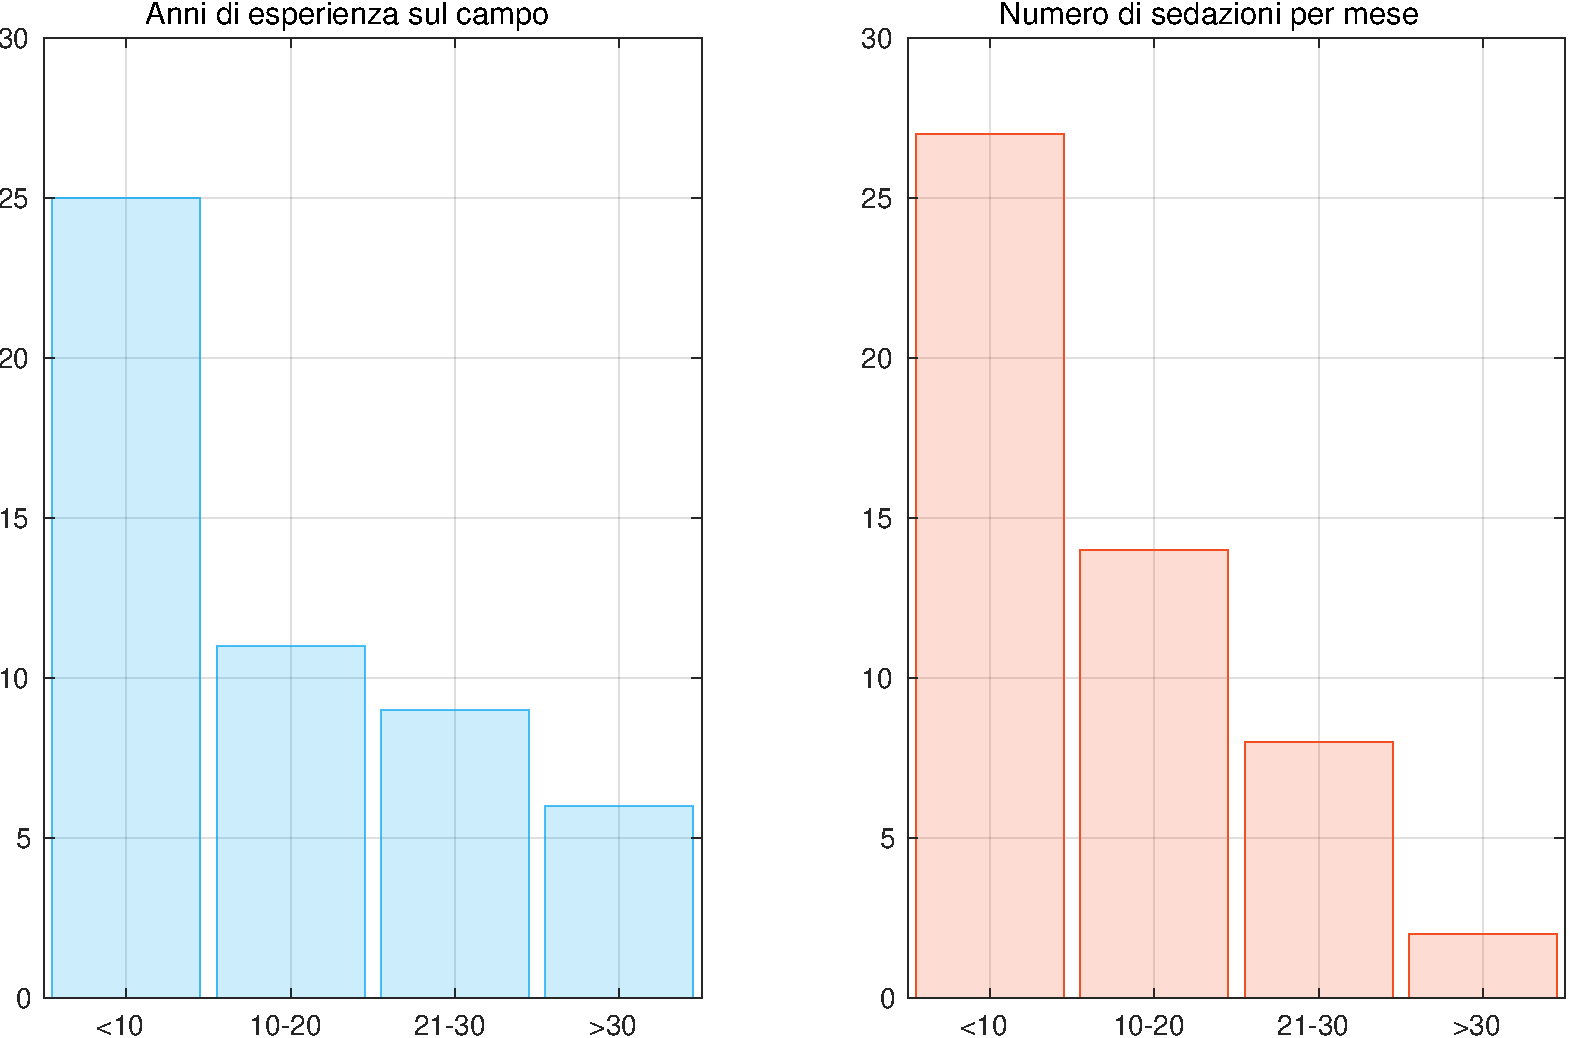
\includegraphics[width=0.9\textwidth]{Figure/esperienzaVSfrequenza.pdf}
    \caption{Anni di esperienza nel campo delle sedazioni procedurali e numero di sedazioni mensilmente assistite.}
    \label{fig:esperienzavsfrequenza}
\end{figure}

\subsection*{Qualità globale della sedazione}
Gli infermieri intervistati hanno dato una valutazione elevata a quasi tutti i farmaci testati: in particolare 32 partecipanti hanno attribuito un punteggio\footnote{Il grado di soddisfazione è stato misurato secondo scala \texttt{NRS}, da 0 a 10.} $\geq$8 alla qualità della sedazione con il propofol, 26 a quella con il midazolam, 23 a quella con la dexmedetomidina. I livelli di soddisfazione più bassi sono stati riscontrati con l'utilizzo della ketamina, infatti solo 8 persone hanno assegnato un punteggio $\geq$8. Nella figura \ref{fig:qualitascolorful} si possono osservare i valori della mediana, del primo e del terzo quartile relativi al livello di soddisfazione percepito dal personale infermieristico, riportati anche numericamente nella tabella \ref{tab:qualitased}: si evince una differenza statisticamente significativa tra le mediane dei punteggi per i differenti farmaci sedativi ed analgesici (Kruskal-Wallis p-value 0.005), in particolare la ketamina ha mostrato un valore significativamente inferiore rispetto al propofol (p-value Bonferroni <0.001), al midazolam (p-value Bonferroni 0.005) ed alla dexmedetomidina (p-value Bonferroni 0.003).

\begin{figure}[h]
    \centering
    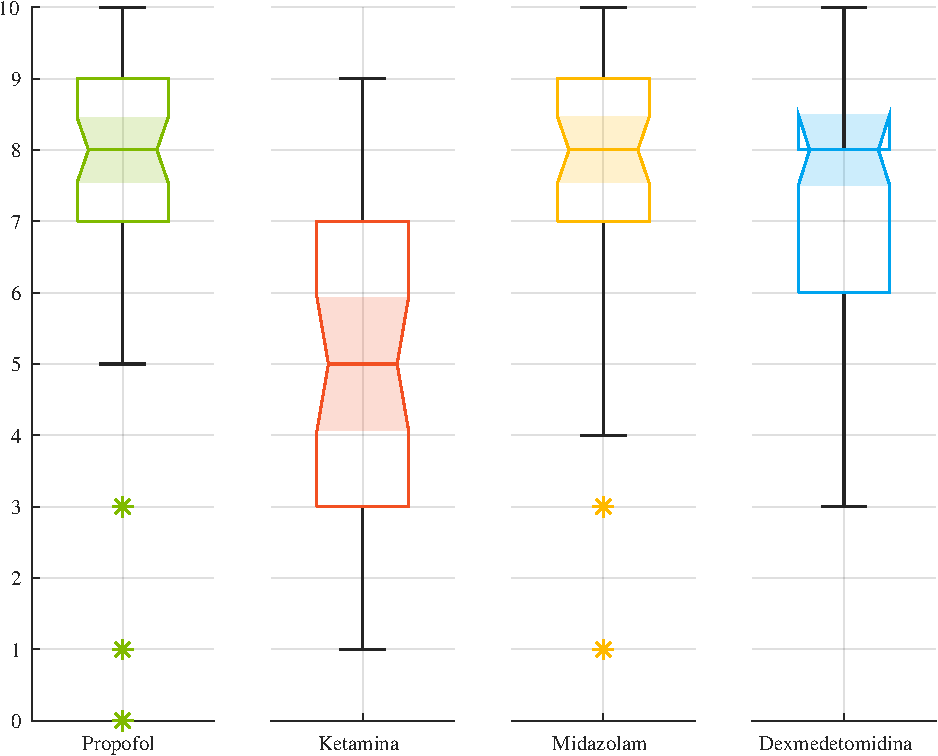
\includegraphics[width=0.9\textwidth]{Figure/qualita-colorful.pdf}
    \caption{Confronto del livello di soddisfazione percepito dagli infermieri (misurato in scala \texttt{NRS}) in relazione ai quattro agenti farmacologici testati in questo lavoro di tesi.}
    \label{fig:qualitascolorful}
\end{figure}

\bgroup
\def\arraystretch{1.5}
\begin{table}[h]
    \centering
    \begin{tabular}{|l|l|}
         Regimi farmacologici & Mediana (IQR) \\ \hline
       Propofol & 8 (7-9)  \\
       Ketamina & 5 (3-7) \\
       Midazolam & 8 (7-9) \\
       Dexmedetomidina & 8 (6-8) 
    \end{tabular}
    \caption{Valori di mediana e quartili associati alla qualità complessiva della sedazione con i quattro agenti farmacologici.}
    \label{tab:qualitased}
\end{table}
\egroup

\subsection*{Correlazione lineare tra esperienza e preferenze farmacologiche}

Stratificando il grado di soddisfazione percepito dal personale infermieristico con gli anni di esperienza compiuti nel campo delle sedazioni procedurali o con il numero di sedazioni mensilmente effettuate non risultano differenze statisticamente significative, come graficamente visibile nelle figure \ref{fig:qualitaesperienza} e \ref {fig:qualitafrequenza}.

\begin{figure}[h]
    \centering
    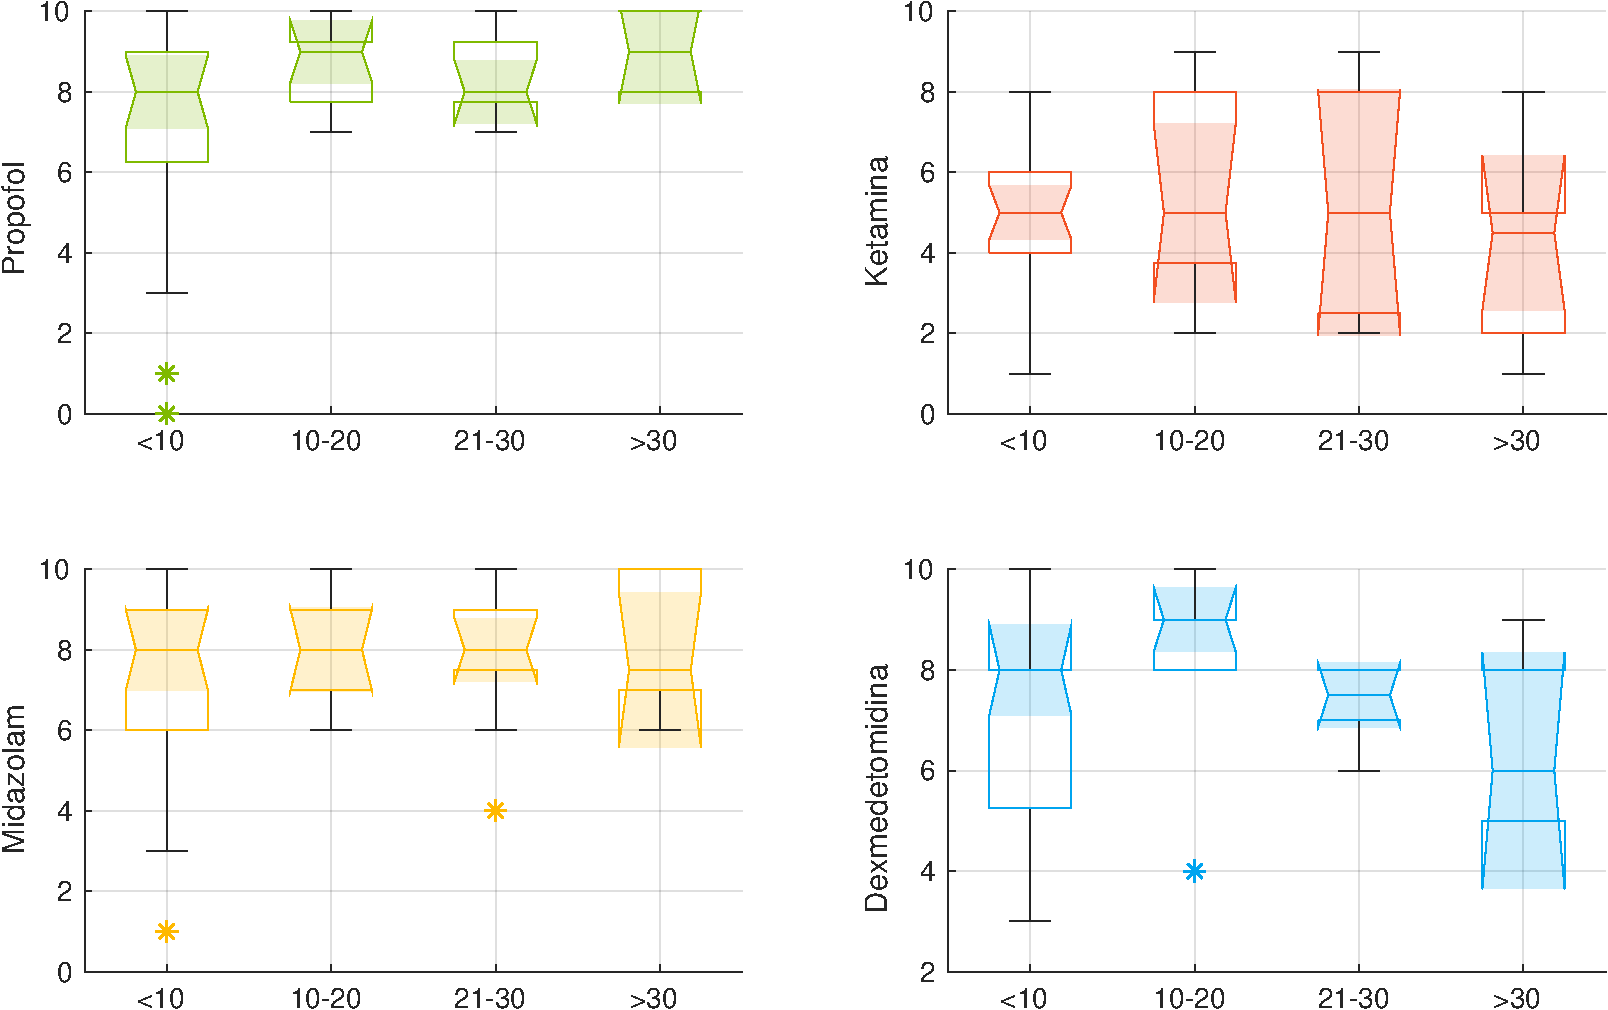
\includegraphics[width=0.9\textwidth]{Figure/qualita-strat-esperienza.pdf}
    \caption{Livello di soddisfazione associato ai diversi agenti farmacologici (misurato secondo scala NRS) stratificato per gli anni di esperienza dei partecipanti nell'ambito delle sedazioni procedurali.}
    \label{fig:qualitaesperienza}
\end{figure}

\begin{figure}[!h]
    \centering
    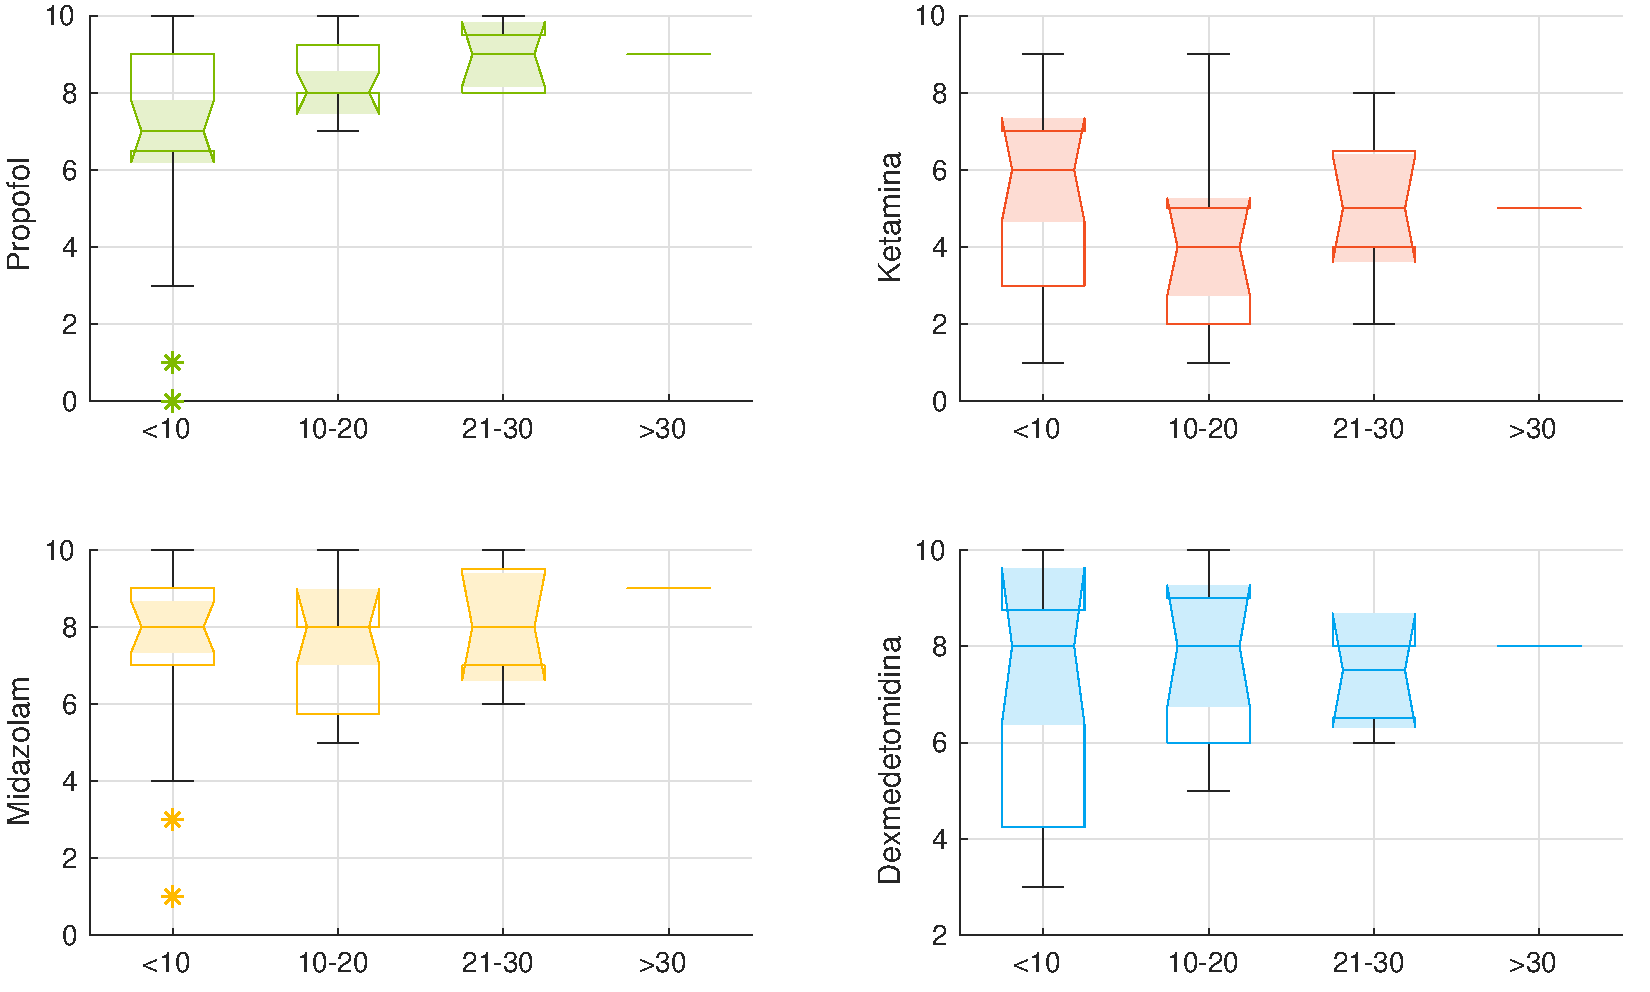
\includegraphics[width=0.9\textwidth]{Figure/qualita-strat-frequenza.pdf}
    \caption{Livello di soddisfazione associato ai diversi agenti farmacologici (misurato secondo scala NRS) stratificato per il numero di sedazioni mensilmente assistite dagli intervistati.}
    \label{fig:qualitafrequenza}
\end{figure}


\subsection*{Grado di sicurezza percepito ed effetti avversi}

Il livello di sicurezza percepito durante la sedazione è risultato elevato per tutti i farmaci testati, senza alcuna differenza statisticamente significativa (Kruskal-Wallis p-value 0.08). I risultati sono rappresentati nella figura \ref{fig:sicurezza} e i valori di mediana e IQR descritti nella tabella\footnote{I dati numerici sono ottenuti attribuendo un valore pari ad 1 alla risposta \emph{per niente}, pari a 6 a \emph{poco}, pari a 10 a \emph{molto}.} \ref{tab:sicurezzased}.

\begin{figure}[!h]
    \centering
    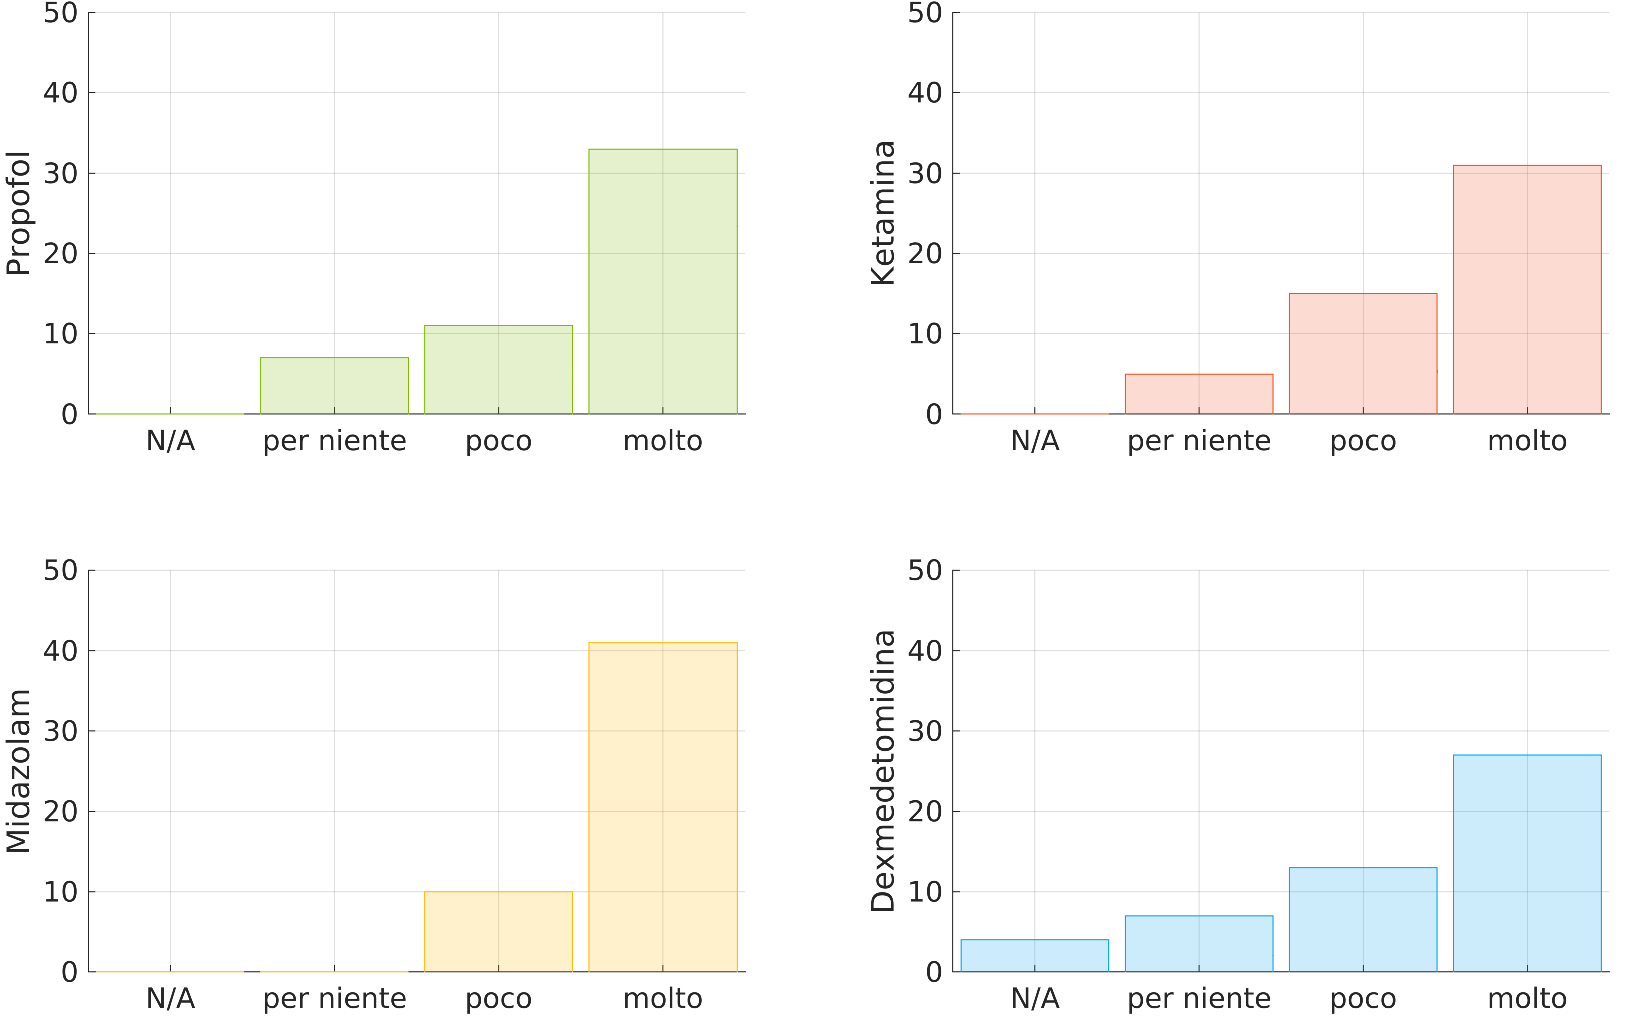
\includegraphics[width=0.9\textwidth]{Figure/sicurezza.pdf}
    \caption{Le risposte del personale infermieristico alla domanda "Quanto ti senti sicuro durante la sedazione con i seguenti farmaci?"}
    \label{fig:sicurezza}
\end{figure}

\bgroup
\def\arraystretch{1.5}
\begin{table}[h]
    \centering
    \begin{tabular}{|l|l|}
         Regimi farmacologici & Mediana (IQR) \\ \hline
       Propofol & 8 (7-9)  \\
       Ketamina & 8 (6-9) \\
       Midazolam & 9 (7-9.5) \\
       Dexmedetomidina & 7.5 (4-8) 
    \end{tabular}
    \caption{Valori di mediana e quartili associati alla sicurezza percepita durante la sedazione con i quattro agenti farmacologici.}
    \label{tab:sicurezzased}
\end{table}
\egroup

Inoltre, la necessità di utilizzare farmaci \emph{rescue} (principalmente antiemetici per la nausea ed il vomito, flumazenil per il \emph{midazolam-induced paradox phenomenon} o infusione di soluzioni contenenti glucosio per evitare eventuali ipoglicemie, soprattutto nei pazienti più piccoli, in caso di tempi di risveglio prolungati) è stata associata da 40 infermieri alla sedazione con ketamina, da 16 a quella con midazolam e da 5 a quella con propofol.

\begin{figure}[!h]
    \centering
    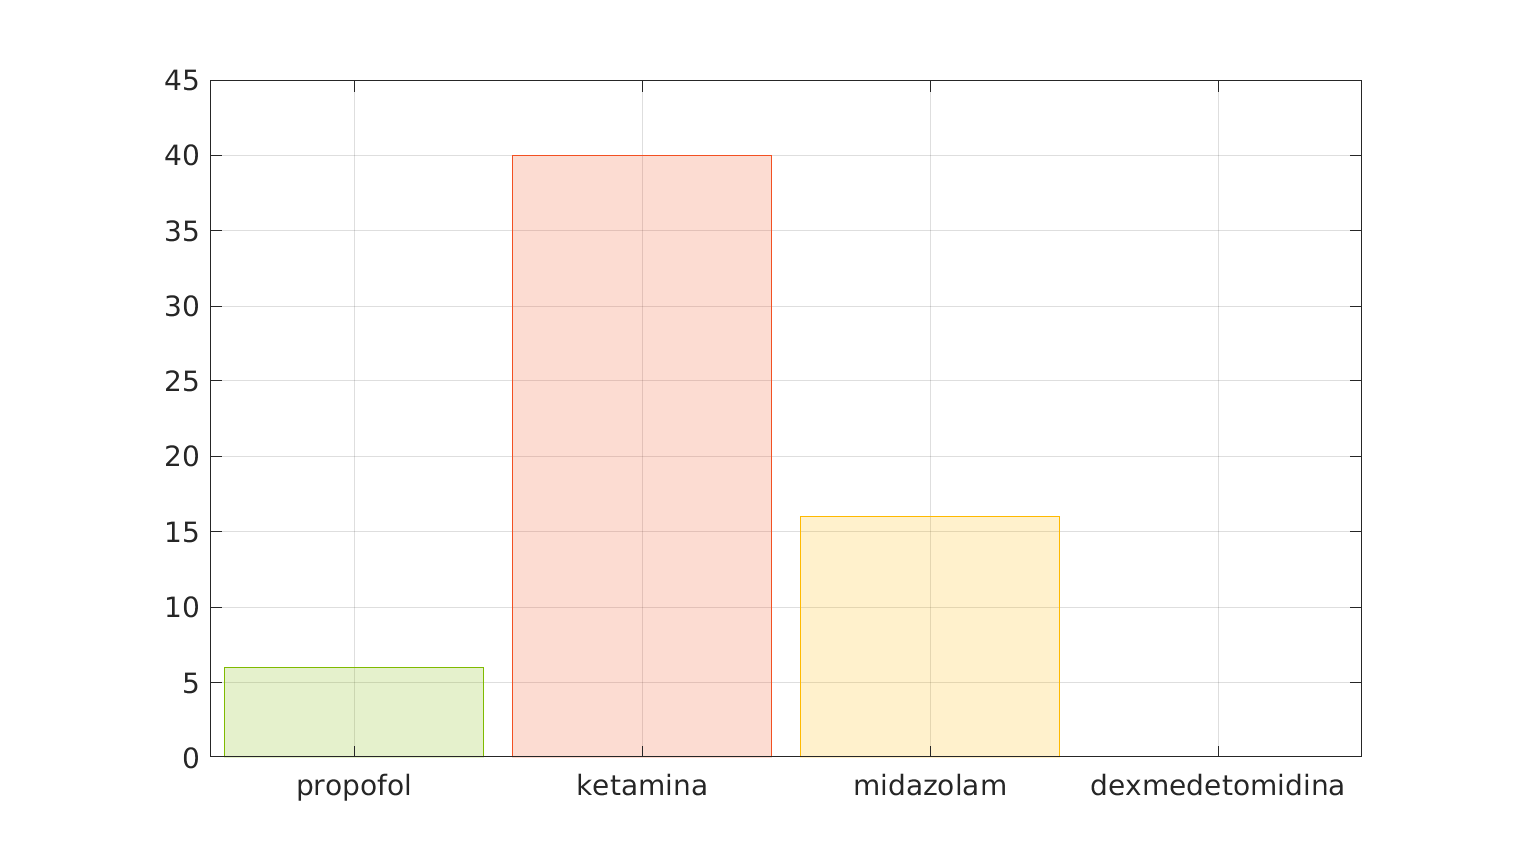
\includegraphics[width=1\textwidth]{Figure/rescue.eps}
    \caption{Risposta alla domanda "Per quali di queste sedazioni è spesso necessario somministrare al risveglio un farmaco \emph{rescue} o sintomatico?"}
    \label{fig:rescue}
\end{figure}

\subsection*{Elementi che influenzano il grado di soddisfazione}

Al fine di comprendere al meglio i motivi alla base delle risposte riportate dagli infermieri aderenti allo studio, è stato chiesto loro di indicare quali aspetti del processo di sedazione hanno influenzato maggiormente il loro giudizio sulla qualità. Quasi tutti (90$\%$) hanno riferito che il proprio grado di soddisfazione è stato influenzato negativamente sia dalla presenza di effetti avversi, sia dall'insoddisfazione del bambino e/o della famiglia; mentre il tipo di farmaco utilizzato, la via di somministrazione, la qualità e il tempo di risveglio, la necessità di ricorrere a farmaci \emph{rescue} e l'impegno infermieristico sono fattori che hanno influito marginalmente alla valutazione finale.
Oltre a ciò, è stato domandato quanto l'incidenza dei possibili effetti collaterali pesi negativamente sul livello di soddisfazione derivato dalla scelta dei diversi sedativi ed analgesici: è emerso che l'insorgenza di distress respiratorio costituisce l'elemento che influisce maggiormente sul giudizio degli infermieri; mentre la manifestazione di nausea o vomito, vertigini, allucinazioni, iperattività od irritabilità esercita un'influenza moderata; infine, la presenza di sonnolenza, incoordinazione motoria, cefalea e alterazioni dell'appetito risulta meno rilevante ai fini del livello di soddisfazione globale percepito. 

\begin{figure}[h]
    \centering
    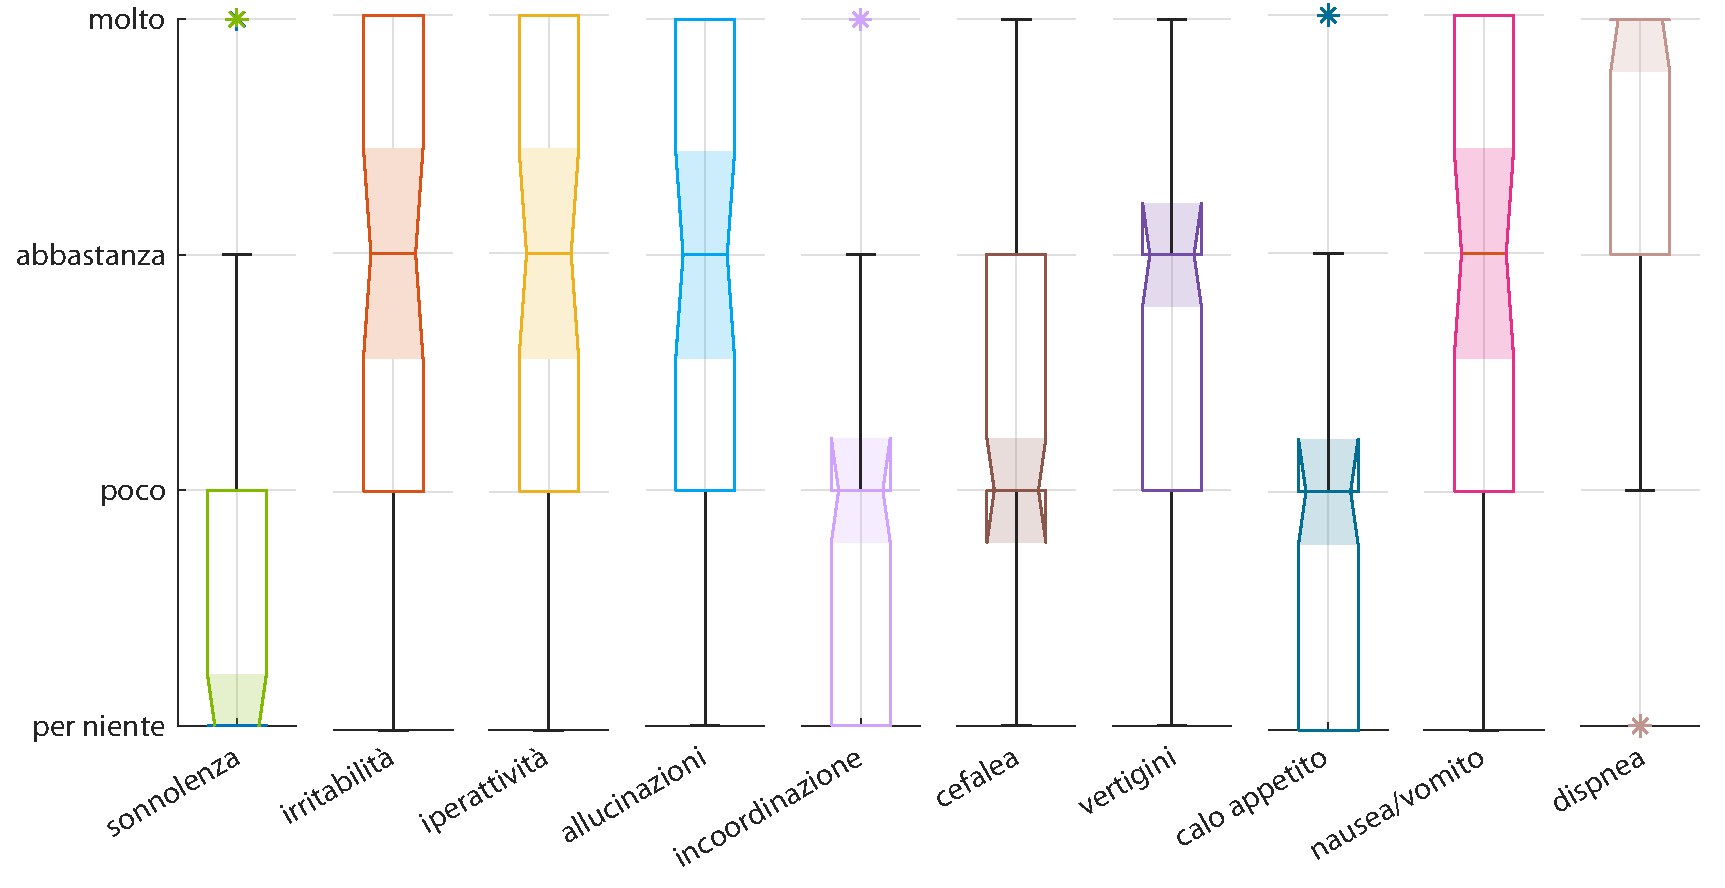
\includegraphics[width=0.9\textwidth]{Figure/influenza-effetti.pdf}
    \caption{Risposta alla domanda "Quanto i seguenti effetti collaterali riducono la tua soddisfazione in merito alla sedazione procedurale?"}
    \label{fig:influenzaeffetti}
\end{figure}


\newpage

\subsection*{Preferenze relative alle vie di somministrazione}

Le vie di somministrazione favorite dagli infermieri sono, in ordine di preferenza: via endovenosa (scelta da 28 persone - 55$\%$), via orale più intranasale (15 - 29.5$\%$), via intranasale (7 - 13.5$\%$) e via intramuscolare (1 - 2$\%$). Inoltre, 40 infermieri (78.4$\%$) vorrebbero che un accesso venoso venisse posizionato abitualmente ed indiscriminatamente in tutti i bambini, mentre 11 (21.6$\%$) desiderano che sia inserito almeno nei casi più difficili, ad esempio nei pazienti con condizioni genetiche note, autismo, ritardo psicomotorio o un alto DIVA score\footnote{\emph{Difficult Intravenous Access score}: si tratta di un sistema di punteggio basato su criteri clinici facili da applicare, che permettono di predire la difficoltà di inserzione del catetere venoso periferico per ciascun paziente pediatrico \cite{Yen2008}.}. Nessun infermiere ha risposto che preferirebbe non venisse mai applicato il cateterismo venoso periferico. 

\begin{figure}[!h]
    \centering
    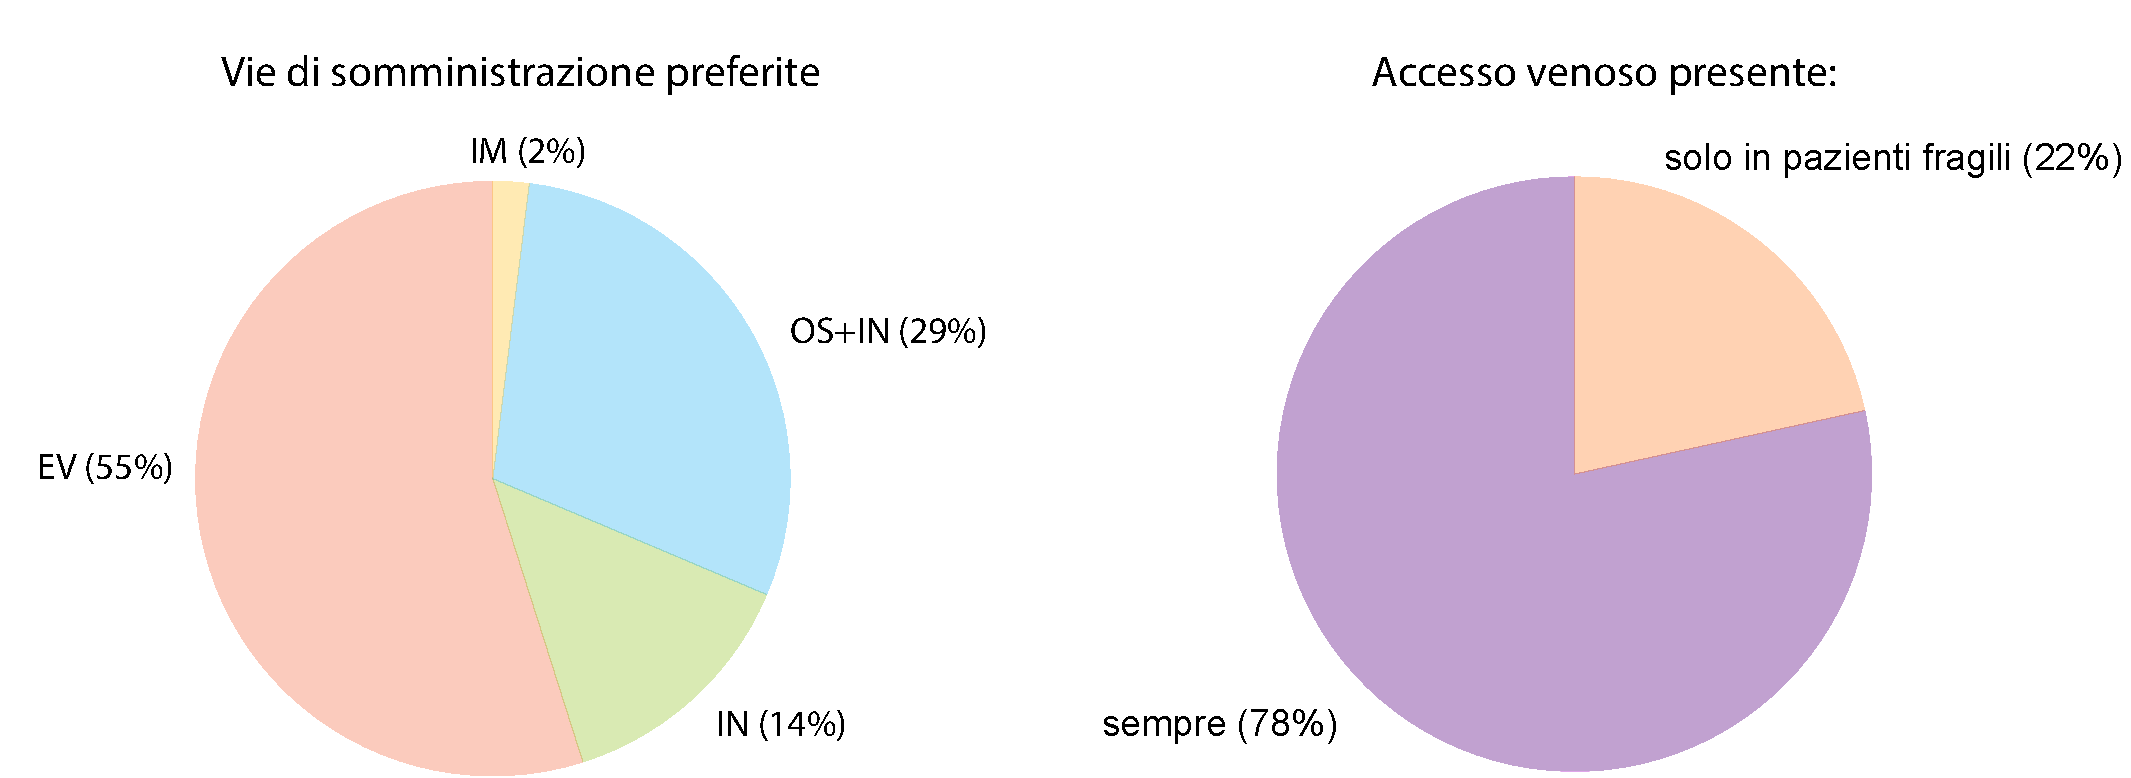
\includegraphics[width=1\textwidth]{Figure/sommicrosoftchiaro.pdf}
    \caption{Vie di somministrazione più apprezzate dagli infermieri per la sedazione procedurale e preferenze relative alla presenza o meno dell'accesso venoso.}
    \label{fig:viedisomm}
\end{figure}


\subsection*{Importanza dell'approccio non farmacologico}

Le tecniche di distrazione attuate prima e durante le sedazioni procedurali sono state giudicate molto importanti da parte di 31 infermieri (60.8$\%$), importanti da 7 (13.7$\%$), poco rilevanti da 9 (17.6$\%$) e non importanti da 4 (7.9$\%$).

\begin{figure}[!h]
    \centering
    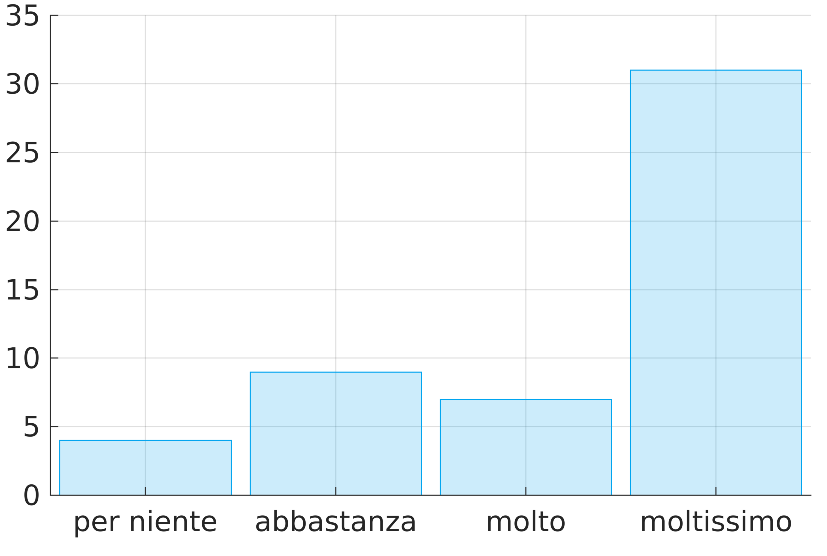
\includegraphics[width=0.6\textwidth]{Figure/distrazione.pdf}
    \caption{Risposta alla domanda "Quanto ritieni utile l’utilizzo di tecniche di distrazione nei bambini per l’esecuzione di procedure non dolorose/minimamente dolorose?"}
    \label{fig:distrazione}
\end{figure}

\subsection*{Suggerimenti per migliorare lo standard di cura attuale}

In conclusione al questionario, è stata data la possibilità di esporre eventuali modifiche che ciascun partecipante attuerebbe nella propria Unità Operativa rispetto agli attuali standard di analgosedazione. A tal proposito è emerso che la maggior parte degli infermieri vorrebbe che venissero realizzati con maggior frequenza dei corsi di formazione ed aggiornamento, inoltre è stato suggerito di implementare ulteriormente l'approccio non farmacologico e di migliorare la qualità della comunicazione tra personale medico ed infermieristico. 